\paragraph{Parameters}

Functions often have \emph{parameters}. When calling the function, we supply \emph{values} for these parameters, which is called \emph{parameter passing}. From the function's perspective, these values are assigned names that are specified in the \emph{parameter list} of the function definition.

\begin{verbatim}
def <name of function>(<parameter list>):
    <function body>
\end{verbatim}

Now consider these two function definitions. Both have two parameters named in their respective parameter lists.

\begin{figure}[h]
\begin{subfigure}[b]{.5\linewidth}
\begin{verbatim}
def date_1(day, month):
    print(day)
    print(month)
\end{verbatim}
\end{subfigure}
\begin{subfigure}[b]{.5\linewidth}
\begin{verbatim}
def date_2(month, day):
    print(day)
    print(month)
\end{verbatim}
\end{subfigure}
\end{figure}

In the left definition we specify the parameters \texttt{day} and \texttt{month}. In the right definition, we specify \texttt{month} and \texttt{day}, in reverse order. This \emph{order} has an effect on what names are given to the values that are passed when calling the function. Let's call the functions:

\begin{figure}[h]
\begin{subfigure}[b]{.5\linewidth}
\begin{verbatim}
date_1(21, 6)
\end{verbatim}
\end{subfigure}
\begin{subfigure}[b]{.5\linewidth}
\begin{verbatim}
date_2(6, 21)
\end{verbatim}
\end{subfigure}
\end{figure}

The output of the functions would then be:

\begin{figure}[h]
\begin{subfigure}[b]{.5\linewidth}
\begin{verbatim}
21
6
\end{verbatim}
\end{subfigure}
\begin{subfigure}[b]{.5\linewidth}
\begin{verbatim}
21
6
\end{verbatim}
\end{subfigure}
\end{figure}

\paragraph{Tracing}

Keeping track of all values when passing parameters can easily become very tedious, which is why we often need to trace them explicitly. Below, like before, we put a line next to the one function that is defined. We also mark the starting line with a little arrow.

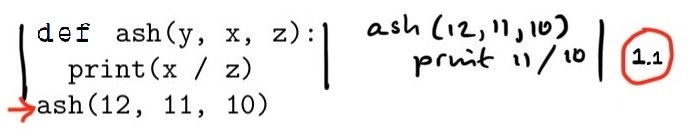
\includegraphics[width=.8\textwidth]{2-trace-params.jpeg}

On that starting line, the function \texttt{ash} is called. To the right of the definition of that function, we draw a line, and copy the function definition, while substituting the concrete values from the \emph{function call}.

Combining the original function definition and the substituted version, we can infer that in the function \texttt{y = 12}, \texttt{x = 11} and \texttt{z = 10}. We use this information to substitute the values of \texttt{x} and \texttt{z} on the line containing \texttt{print}.

Then, only one calculation is left, the result of which will be printed. When we evaluate the expression, we get the number that will be printed: \texttt{1.1}.
